 \section{Introduction}
\label{sec:intro}

% basic introduction to table linking
The World Wide Web is endowed with billions of HTML tables,
i.e. web tables~\cite{cafarella2008webtables,wang2012understanding}, which carry
valuable structured information. To enable machines to understand and process 
such tables~\cite{wang2012understanding},
the first step is to link the surface mentions of the entities in the 
tables to a standard lexicon or knowledge base, such as Wikipedia, which 
uniquely identifies entities. This task is
known as entity linking in web tables~\cite{bhagavatula2015tabel,wu2016entity}.
In this paper, we also call it ``table linking''.
%Because most of the existing well-known knowledge bases maintain entries primarily in English,

Existing work has been focused on entity linking for web tables 
in English~\cite{bhagavatula2015tabel,limaye2010annotating}, or mono-lingual table linking.
However, when it comes to linking web tables in other languages, the corresponding
non-English knowledge bases are often not comprehensive enough to cover all the entity mentions 
in the tables at hand.  The Chinese Wikipedia, for instance, is just about 1/6 the size of
its English counterpart, in terms of the number of entities (articles). This motivates us to
link non-English web tables to English knowledge base, in a novel process 
that we call {\em cross-lingual table linking}.
For example, the movie ``
%邮差
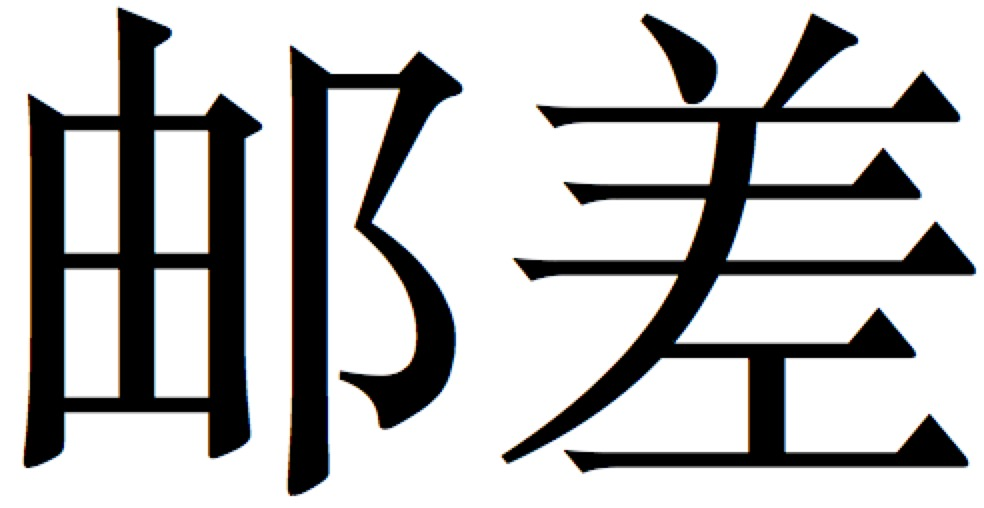
\includegraphics[height=1.3\fontcharht\font`\B]{figures/youchai.png} 
'' (Postman) in a Chinese table in 
\figref{fig:chinesetable} is not included in the Chinese Wikipedia but available in 
the English version. Thus, we can link  ``
%邮差
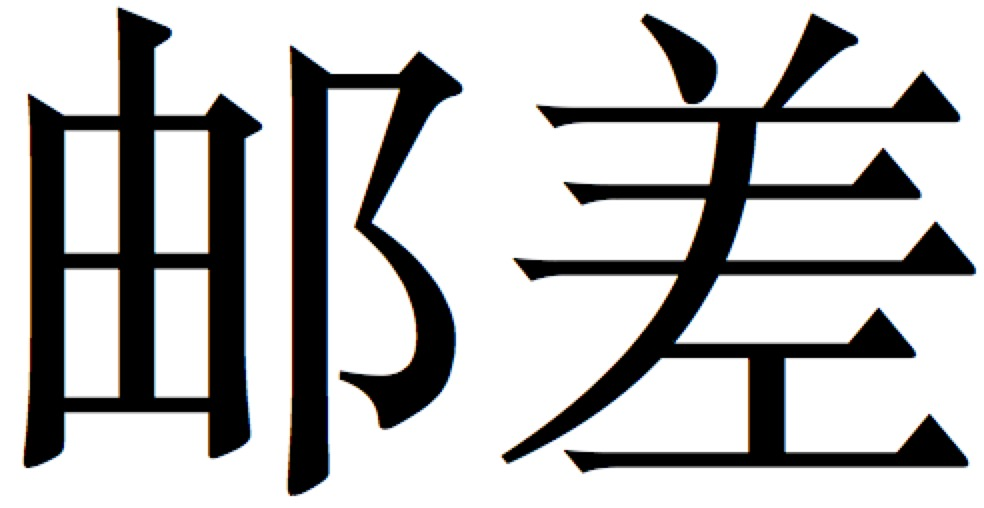
\includegraphics[height=1.3\fontcharht\font`\B]{figures/youchai.png} 
'' to ``Il Postino: The Postman'' in the English Wikipedia.

Another important motivation for cross-lingual table linking is to 
help enrich the facts in the target knowledge base. 
Knowledge bases in English,  albeit larger and better structured than those in other languages,
may contain long-tail entities. These are entities associated with very few attributes 
or relations in the KB, such as Chinese movies or celebrities, since such information is often
ignored by the English-speaking Wiki contributors.
%and is well-formed in the structure,
%but rare attributes or relationships are attached to long-tail entities like Chinese movies or celebrities,
%as the information of which mainly comes from Chinese communities.
%Meanwhile, the structure of the web table enables discovering semantic relationships between cells in a row or column.
On the other hand, non-English web tables may be a rich source of 
semantic relationships among these rare entities.
For example, the table in \figref{fig:chinesetable} contains the relationship between movies and
their countries of origin. ``
%线人

\includegraphics[height=1.3\fontcharht\font`\B]{figures/xianren.png} 
''(informant) is a Chinese movie that exists in English Wikipedia
(``The\_Stool\_Piegon\_(2010\_film)'') and hence Freebase, but it misses a property 
{\em film\_country}. Now if we can link the mentions in the table to the correct entities in
English Wikipedia, then it is easy to infer that the {\em film\_country} property of 
``The\_Stool\_Piegon\_(2010\_film)'' is China, thus discovering a new fact. 

%mentions of each row represents a film, its genre and the country of production.
%Once mentions in the Chinese table are correctly linked,
%we are able to learn the hidden semantics in the table and enrich the backend knowledge base,
%which is benifitical to both popular entities like ``钢铁侠'' (``\textit{Iron\_Man\_(2008\_film)}''),
%and long-tailed entities like the Chinese film ``线人'' (``\textit{The\_Stool\_Piegon\_(2010\_film)}'').
%%For example, information extracted from a table about Chinese celebrities can be
%used to enrich knowledge in Freebase or IMDB.
%On the other hand, since knowledge bases in English are more
%comprehensive and accurate than that of other languages,
%entity linking systems in foreign languages often fail to identify 
%an entity due to incompleteness of KB in their languages.
%Incorporating English entities into the target KB can improve 
%the recall of entity linking systems in such cases.
%\KZ{The above reason seems not compelling enough to make the following
%claim.}
%Therefore, there is a substantial need to link entities in 
%non-English web tables
%to English knowledge bases. \figref{fig:chinesetable} depicts such a scenario. 
%After cross-lingual table linking, ``钢铁侠'' in the second row is linked to its 
%corresponding real world entity \textit{Iron Man (2008 film)} in a KB (e.g., Freebase). \KQ{WIKIPEDIA}

\begin{figure}[th]
\centering
\scalebox{0.22}{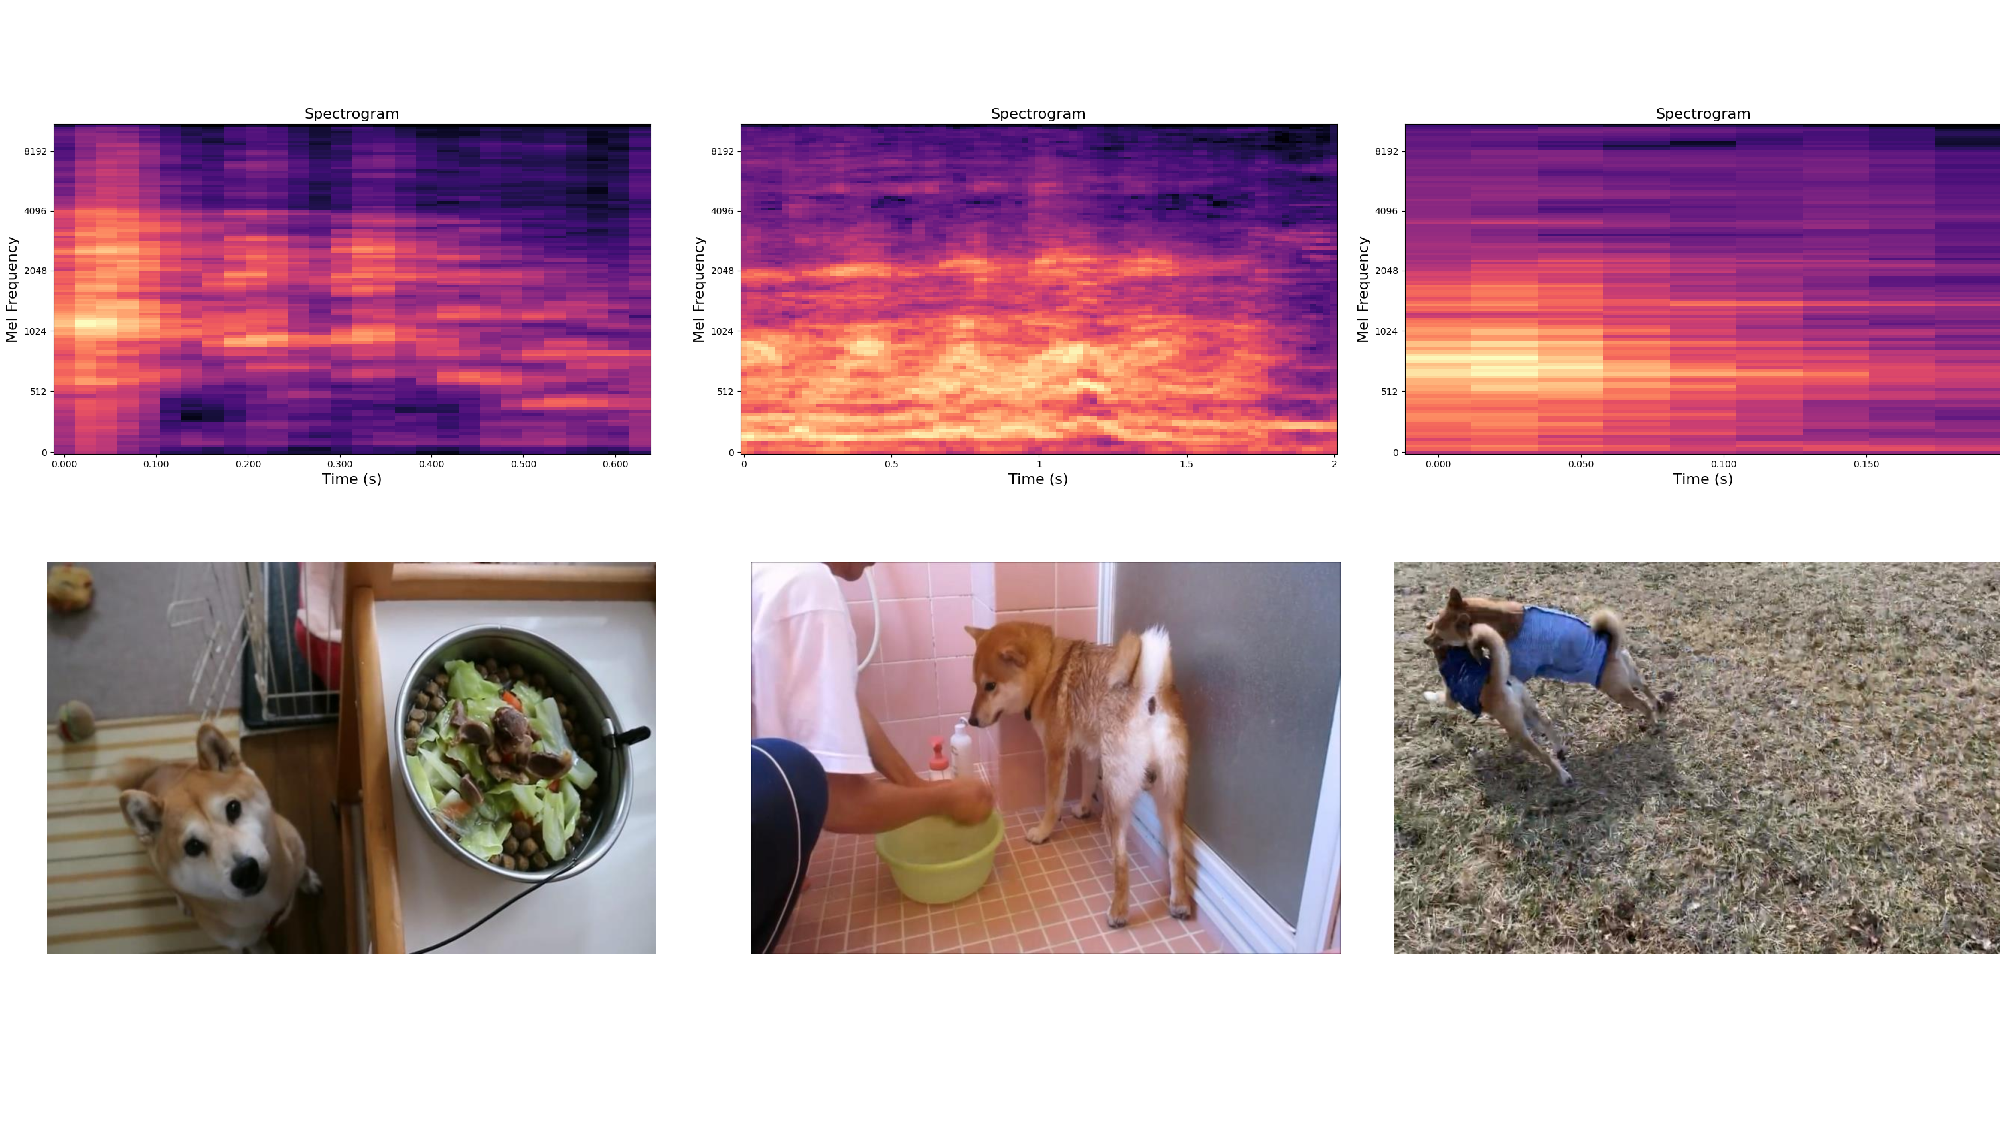
\includegraphics[angle=0]{figures/intro_example.pdf}}
%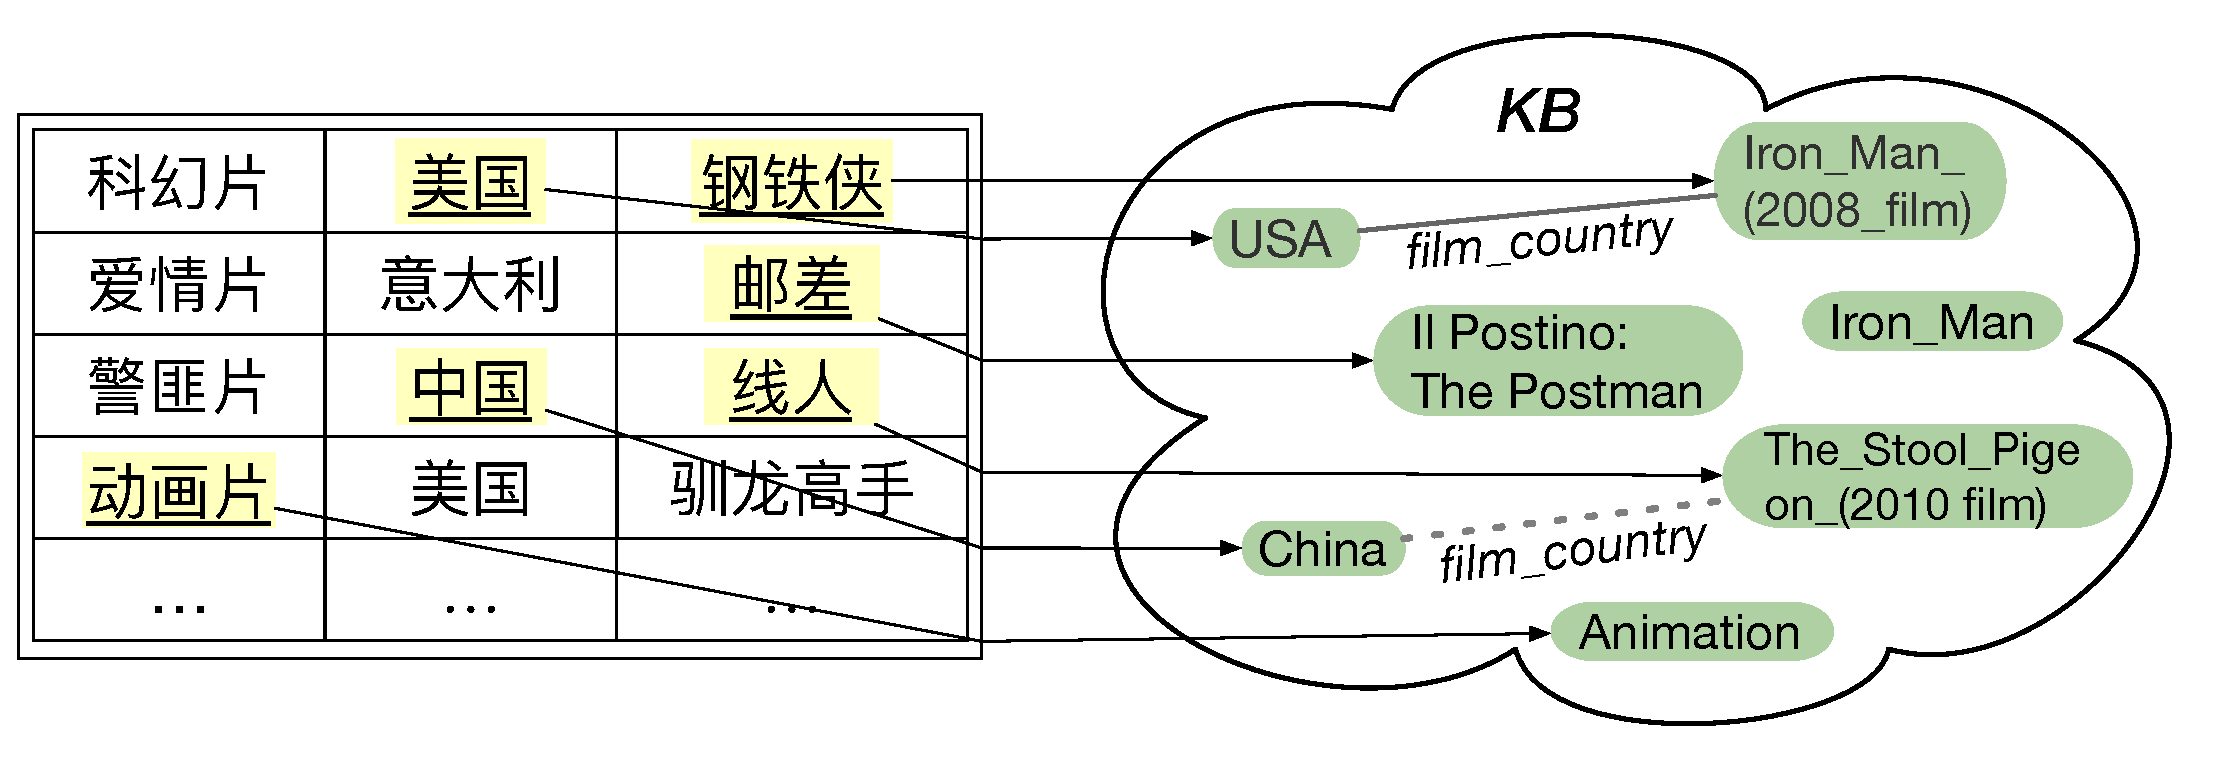
\epsfig{file=figures/intro_example.eps, angle=0, width=1.0\columnwidth}
\caption{Example of cross-lingual table linking from Chinese to English.}
\label{fig:chinesetable}
\end{figure}

In this paper, we attempt to solve the cross-lingual table linking problem
{\em without} using any non-English knowledge bases.
%That is, our goal is to link the mentions in the non-English table 
%directly to an entity in the English knowledge base. 
%The advantage of this is we do not discard any information of non-English mentions
%so that our model has the ability to tolerate the error caused by translation.
To the best of our knowledge, this is the first attempt that attacks the 
cross-lingual table linking problem. 


There are two naive approaches to accomplish this cross-lingual table linking task.
In the first approach, one can use any of the mono-lingual table linking techniques developed thus far
to first link the entities to a knowledge base of that language, and then link to
the English knowledge base via inter-language links~\cite{tsai2016cross}.
For example, Wikipedia provides such inter-language links. 
This approach may not work because i) the non-English knowledge base 
may not have all the entities in tables; and ii)
many non-English knowledge sources provide no inter-language links. 

In the second approach, one can directly translate all the entity names in
the non-English web table into English,
and then use the mono-lingual table linking techniques to link to 
an English knowledge base~\cite{mcnamee2011cross}.
This two-step approach is also not effective because
it is analogous to a distant supervised learning,
where the association between non-English names and English entities are not directly available for training.
If the translation is wrong, the error will propagate in the following linking steps.


%The key step of converting Web tables into machine-readable knowledge 
%is entity linking, which refers to a task of mapping the mentions in table cells to the referent entities in a Knowledge Base (KB), such as Freebase and Wikipedia. 
% add some example

% However... non-English KB is not good enough, give some examples.
%Most widely used KBs are written in English. KBs in other languages suffer backwards at both size and quality. For example, The latest English Wikipedia contains XXXX articles while Chinese version only has a size of XXXX.\XS{say sth about quality} In the meantime, the percentage of Web pages written in English are decreasing due to widely development of Web technology accross different cultures. Thus, it becomes more and more important to maintain the growth of KBs by absorbing infomation from all Web contexts of different languages. In the previous example, the table could be in a Chinese article so the mention to link  is ``XXX'' instead. We call this new task as cross lingual table linking.

% Challenges, table -> no contexts, language -> gap 
% First try on cross lingual table linking
%There are various efforts \XS{cite} trying to solve entity linking task 
%for Web tables while no one ever makes an attempt under cross lingual environment.

In any approach to entity linking (mono- or cross-lingual), 
a necessary step is to generate a set of candidate entities
~\cite{tsai2016cross,mcnamee2011cross,bhagavatula2015tabel,wu2016entity},
and then the problem is transformed to a ranking problem, which aims to pick
the entity that is most similar to the mention in the table. 
%The similarity computation requires the feature representation for a mention to be 
%compatible with the representation for an entity. 
The major technical challenge of our task is since the source mention
and the target entity come from two different languages,
their feature representations are naturally incompatible. 
To make matters worse, tables offer very limited context for disambiguating
a mention in the first place.

%Since the language of source mention and target entity is inconsistent, 
%it's hard to direct use the surrounding infomation of them \XS{rephrase}. 
%Besides, this task still has to face a lack of surrounding contexts 
%which can be very helpful during entity disambiguation in normal entity linking tasks.

% image CNN, table is like image
We thus propose a neural network based joint model for cross-lingual table linking. 
We embed mention, context and entity in a continuous vector space to 
capture their semantics.
Further, we employ a linear transformation between vector spaces of two languages. 
For each table, we link all the mentions simultaneously, 
so as to fully utilize the relationships among entities 
in the same row or column. We encode these correlations as a 
{\em coherence} feature in the model.
Furthermore, we design a pairwise ranking loss function for parameter 
learning and propose an iterative prediction algorithm to link new tables.


%Most existing work \XS{cite} mines hand-crafted features to measure the similarity 
%between mentions and candidate entities.  Since feature engineering suffers XXX, 
%some work attempt to use nerual network \XS{cite} to generate fearures, 
%which shows great improvements in task of entity linking. 
%
%As we should notice, a table can be regarded as a matrix of texts, similar to an image, which is a matrix of pixels. 
%Inspired by that idea of using deep neural networks to capture rich semantics of images, which has been proven successful, 
%we present a jointly modeling framework based on nerual networks to solve our problem.
%Besides, Convolotional Neural Networks(CNN) is a natural structure to deal with data in matrix form such as tables.

% Contribution
The contribution of this paper is summarized below.
\begin{itemize}
\itemsep0em
\item We are the first to define the problem of cross-lingual entity linking 
for web tables (\secref{sec:problem});
\item We present a novel neural network based joint model which effectively captures the rich semantics of mention table and referent entity table simultaneously. Based on that, we bridge the gap between different languages in this task (\secref{sec:translation} and \secref{sec:cell});
\item We propose a coherence feature in the joint linking model which captures the correlation of entities appearing in the same table and improves the linking accuracy (\secref{sec:coherence});
\item The framework significantly outperforms
several baseline methods, with an accuracy of 62.9\%. (\secref{sec:eval}).
%and question answering. Furthermore, our schema representation is
%on par with the popular word embedding model in computing relation similarity (\secref{sec:eval}).
\end{itemize}
